%!TEX encoding = UTF-8 Unicode
%!TEX root = ../lect-w09.tex

%%%


%\begin{Slide}{TODO: Begrepp att förklara}
%  Tänk igenom ordningen:
%  \begin{itemize}
%    \item OO, arv, supertyp, subtyp, bastyp, polymorfism, ...
%  \end{itemize}
%\end{Slide}


\Subsection{Överskuggingsregler, \texttt{override}}

\begin{Slide}{Medlemmar, arv och överskuggning}\SlideFontTiny
\begin{multicols}{2}
Olika sorters överskuggningsbara medlemmar i klasser och traits i \Emph{Scala}:
\begin{itemize}
\item \code{def}
\item \code{val}
\item \code{lazy val}
\item \code{var}
\end{itemize}


\columnbreak

\pause

Olika sorters överskuggningsbara instansmedlemmar i \Emph{Java}:
\begin{itemize}
\item variabel
\item metod
\end{itemize}

{\SlideFontTiny Medlemmar som är \jcode{static} kan ej överskuggas (men döljas) vid arv.}

\vspace{0.5em}
\end{multicols}

\pause
\begin{itemize}\SlideFontTiny
\item När man överskuggar \Eng{override} en medlemmen med en annan medlem med samma namn i en subtyp, får denna medlem en (ny) implementation.

\item När man konstruerar ett objektorienterat språk gäller det att man definierar sunda överskuggningsregler vid arv. Detta är förvånansvärt knepigt.

\item Singelobjekt kan ej ärvas (och medlemmar i singelobjekt kan därmed ej överskuggas).
\end{itemize}
\end{Slide}


\begin{Slide}{Fördjupning: Regler för överskuggning i Scala} \SlideFontTiny
\label{slideW07:overriderules}
En medlem M1 i en supertyp får överskuggas av en medlem M2 i en subtyp, enligt dessa regler:
\begin{enumerate}
\item M1 och M2 ska ha samma namn och typerna ska matcha.
\item \code{def} får bytas ut mot: \code{def}, \code{val}, \code{var}, \code{lazy val}
\item \code{val} får bytas ut mot: \code{val}, och om M1 är abstrakt mot en \code{lazy val}.
\item \code{var} får bara bytas ut mot en \code{var}.
\item \code{lazy val} får bara bytas ut mot en \code{lazy val}.
\item Om en medlem i en supertyp är abstrakt \emph{behöver} man inte använda nyckelordet \code{override} i subtypen. (Men det är bra att göra det ändå så att kompilatorn hjälper dig att kolla att du verkligen överskuggar något.)
\item Om en medlem i en supertyp är konkret \emph{måste} man använda nyckelordet \code{override} i subtypen, annars ges kompileringsfel.
\item M1 får inte vara \code{final}.
\item M1 får inte vara \code{private} eller \code{private[this]}, men kan vara \code{private[X]} om M2 också är \code{private[X]}, eller \code{private[Y]} om X innehåller Y.
\item Om M1 är \code{protected} måste även M2 vara det.

\end{enumerate}
\end{Slide}


\begin{Slide}{Fördjupning: Regler för överskuggning i Java}
\url{http://docs.oracle.com/javase/tutorial/java/IandI/override.html}
\end{Slide}


\Subsection{\texttt{super}}

\begin{Slide}{Att skilja på mitt och ditt med \texttt{super}}
\begin{REPL}
scala> class X { val gurka = "super pepinos" }

scala> class Y extends X {
         override val gurka = ":("
         val sg = super.gurka
       }

scala> val y = new Y
y: Y = Y@26ba2a48

scala> y.gurka
res0: String = :(
\end{REPL}

\pause
Super Pepinos to the rescue:
\begin{REPLnonum}
scala> y.sg
res1: String = super pepinos

\end{REPLnonum}


\pause
\begin{tikzpicture}[overlay]
     \node at (7.5,1.7) {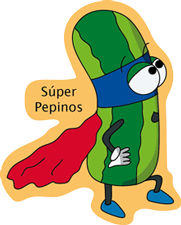
\includegraphics[scale=0.5]{../img/ttsuper}};
\end{tikzpicture}
\href{http://www.pepinadas.com/tirassuper1.html}{\small www.pepinadas.com/tirassuper1.html}
\end{Slide}





\Subsection{Trait eller abstrakt klass?}

\begin{Slide}{Trait eller abstrakt klass?}
\SlideFontSmall
\label{slideW07:traitorclass}
\begin{multicols}{2}
Använd en \Emph{trait} som supertyp om...
\begin{itemize}
\item ...du är osäker på vilket som är bäst. (Du kan alltid ändra till en abstrakt klass senare.)
\item ...du vill kunna mixa in din trait tillsammans med andra traits.
\item ...du vill skapa ett flexibelt gränssnitt som del i ett api.

\end{itemize}

\columnbreak

Använd en \Alert{abstrakt klass} som supertyp om...
\begin{itemize}
\item ...du vill ge supertypen en parameter vid konstruktion.
\item ...du vill ärva supertypen från klasser skrivna i Java.
\item ...du vill minimera vad som behöver omkompileras vid ändringar.
\end{itemize}


\end{multicols}
\end{Slide}



\begin{Slide}{Terminologi och nyckelord vid arv}\SlideFontTiny

\begin{tabular}{r  l}
\Emph{subtyp}           & en typ som ärver en supertyp\\
\Emph{supertyp}         & en typ som ärvs av en subtyp\\
\Emph{bastyp}           & en typ som är rot i ett arvsträd\\
\Emph{abstrakt medlem}  & en medlem som saknar implementation\\
\Emph{konkret medlem}   & en medlem som ej saknar implementation\\
\Emph{abstrakt typ}     & en typ som kan ha abstrakta medlemmar; kan ej instansieras\\
\Emph{konkret typ}      & en typ som ej har abstrakta medlemmar; kan instansieras\\
\code|class|            & en klass är en konkret typ: \Alert{kan ej ha abstrakta medlemmar}\\
\code|abstract class|   & en klass är en abstrakt typ som \Emph{kan ha parametrar}\\
\code|trait|            & är en abstrakt typ, \Alert{kan ej ha parametrar} men \Emph{kan mixas in}\\
\code|extends|          & står före en supertyp, medför arv av supertypens medlemmar\\
\code|override|         & en medlem överskuggar (byter ut) en medlem i en superttyp\\
\code|protected|        & gör en medlem synlig i subtyper till denna typ (jmf \code|private|)\\
\code|final gurka|      & gör medlemen gurka final: förhindrar överskuggning\\
\code|final class|      & gör klassen final: förhindrar vidare subtypning\\
\code|sealed trait|     & förseglad trait: bara de direkta subtyperna i denna kodfil\\
\code|super.gurka|      & refererar till supertypens medlem \code|gurka| (jmf \code|this|)\\
\end{tabular}

\ifkompendium\else
\pause
\begin{tikzpicture}[overlay]
     \node at (10.7,0.6) {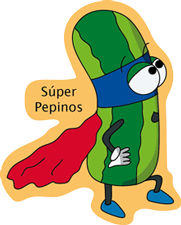
\includegraphics[scale=0.36]{../img/ttsuper}};
\end{tikzpicture}
\fi

\end{Slide}
